\documentclass{article}

% if you need to pass options to natbib, use, e.g.:
% \PassOptionsToPackage{numbers, compress}{natbib}
% before loading nips_2018

% ready for submission
% \usepackage{nips_2018}

% to compile a preprint version, e.g., for submission to arXiv, add
% add the [preprint] option:
\usepackage[preprint]{nips_2018}

% to compile a camera-ready version, add the [final] option, e.g.:
% \usepackage[final]{nips_2018}

% to avoid loading the natbib package, add option nonatbib:
% \usepackage[nonatbib]{nips_2018}

\usepackage[utf8]{inputenc} % allow utf-8 input
\usepackage[T1]{fontenc}    % use 8-bit T1 fonts
\usepackage{hyperref}       % hyperlinks
\usepackage{url}            % simple URL typesetting
\usepackage{booktabs}       % professional-quality tables
\usepackage{amsfonts}       % blackboard math symbols
\usepackage{nicefrac}       % compact symbols for 1/2, etc.
\usepackage{microtype}      % microtypography
\usepackage{graphicx}
\graphicspath{ {./graphics/} }

\title{Solving OpenAI's CarRacing environment using Deep Reinforcement Learning and Dropout}

% The \author macro works with any number of authors. There are two
% commands used to separate the names and addresses of multiple
% authors: \And and \AND.
%
% Using \And between authors leaves it to LaTeX to determine where to
% break the lines. Using \AND forces a line break at that point. So,
% if LaTeX puts 3 of 4 authors names on the first line, and the last
% on the second line, try using \AND instead of \And before the third
% author name.

\author{
  David S.~Hippocampus\thanks{Use footnote for providing further
    information about author (webpage, alternative
    address)---\emph{not} for acknowledging funding agencies.} \\
  Department of Computer Science\\
  Cranberry-Lemon University\\
  Pittsburgh, PA 15213 \\
  \texttt{hippo@cs.cranberry-lemon.edu} \\
  %% examples of more authors
  \And
  Patrik Gerber \\
  University of Oxford \\
  Corpus Christi College, Oxford, UK \\
  \texttt{patrik.gerber@ccc.ox.ac.uk} \\
  %% \AND
  %% Coauthor \\
  %% Affiliation \\
  %% Address \\
  %% \texttt{email} \\
  %% \And
  %% Coauthor \\
  %% Affiliation \\
  %% Address \\
  %% \texttt{email} \\
  %% \And
  %% Coauthor \\
  %% Affiliation \\
  %% Address \\
  %% \texttt{email} \\
}

\begin{document}
% \nipsfinalcopy is no longer used

\maketitle

\begin{abstract}
Deep Reinforcement Learning methods have seen many successes in recent years, ranging from solving classical video games to beating 
world class Go players. However, little progress has been made on the front of generalizability: successful models are trained for 
narrow, well-defined tasks, often using a vast amount of compute time. These models perform well in their specific task, but slight 
perturbations in the environment often cause disproportionate decrease in performance. Regularization methods have not yet been shown 
successful in tackling this issue of overfit. In this paper we attempt to give such a positive example, by applying the DDQN-algorithm 
with Dropout to solve OpenAI's CarRacing environment, using only a small subset of the state space for training. 
\end{abstract}


\section{Introduction}
% The field of Reinforcement Learning (RL) concerns itself with the task of learning from interaction to maximize a reward signal. 
% In the setting of this interaction, the decision maker is called the \textit{agent} and the world it interacts with is called the 
% \textit{environment}. At each time step the \textit{agent} chooses and \textit{action} to take, and the environment responds with 
% resulting \textit{state} of the environment and a scalar \textit{reward} signal. 
\par
OpenAI Gym is a set of Reinforcement Learning testbeds including many classical video games and control problems. OpenAI Gym's 
CarRacing environment - from here on referred to as the 'car racing game' - is a simple, top-down view racing game as shown in 
Figure \ref{fig:carracing}. The agent has control of a race-car, and its goal is to visit the tiles making up the randomly 
generated track, as fast as possible. At each time step, the \textit{reward} is -0.1 if no tile was visited and 
$\frac{1000}{Number\ of\ tiles}$ otherwise. The \textit{state} is represented as 96 by 96 RGB screenshots of the screen. The game 
ends if the agent visits all tiles on the track or the number of passed frames exceeds 1000. This environment is considered solved 
as per OpenAI's guidelines, if an average score of over 900 is achieved over 100 consecutive games. The car racing game was recently 
solved by \cite{World_Models}, however to the best of our knowledge it is unsolved using RL methods. 

In this paper we outline a method that solves the game, trained on a remarkably small subset of the full environment. This is 
achieved using dropout to regularize the convolutional neural network used, showing that 


\begin{figure}
  \centering
  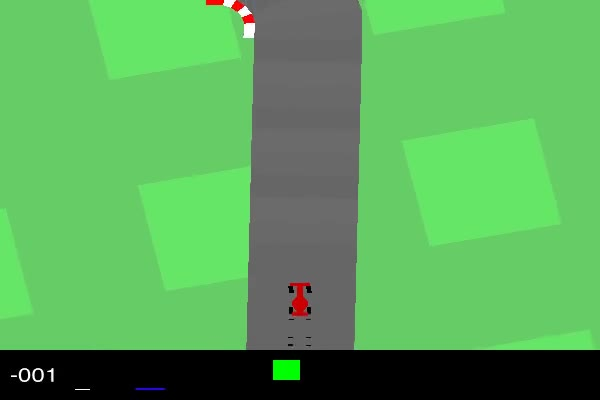
\includegraphics[width=0.5\linewidth]{carracing.jpg}
  \caption{Screenshot of the car racing game. }
  \label{fig:carracing}
\end{figure}

\section{Method}
Our method uses the DDQN-algorithm as first described in \cite{DDQN}, a simple extension of the celebrated DQN-algorithm, 
proposed in \cite{DQN}. The architecture of the Q-network is that described in the original paper \cite{DQN}

\section{Experiments}
Notice that the track is made up of distinct tiles. The reward signal is -0.1 for every frame passed and $\frac{1000}{N}$ for 
every tile visited, where N is the total number of tiles on the track. Thus the goal of the game is to finish the track as 
fast as possible, without missing any of the tiles. The actions come in the form of an array of three numbers. In the array, 
the first number indicates steer, the second number indicates acceleration and the third number indicates deceleration. The 
steer coordinate is continuous from -1 to 1 while the acceleration and the deceleration are continuous from 0 to 1. For example, 
if the agent finishes in 732 frames and never leaves the track doing so, the reward is 1000 - 0.1*732 = 926.8 points. The 
episode finishes when all tiles are visited or more than 1000 frames pass. As per OpenAI's guidelines, the environment is 
solved when an average score of 900 or more is achieved over 100 episodes. 
\par

We chose this environment for several reasons: first, the car racing game is similar to real life autonomous driving; second, the game environment can be easily altered, allowing for interesting exploration of robustness of Deep RL methods; third, according to the leaderboard on OpenAI's website, no one has successfully solved the game. 
\par

To be able to iterate faster, we created four different types of training environment of varying complexity: random short tracks, fixed one track, fixed three tracks and random tracks. In the random short track environment, there are 50 tiles for the agent to finish while in the other environments, there are approximately 300 tiles. Random short tracks and random tracks environment display randomly generated tracks for each episode while the other environments display the same one (fixed one track) or three tracks (fixed three tracks).

\section{Results}

\section{Conclusion}

% -------------------------------------------------------------------------------------------------------------------
% -------------------------------------------------------------------------------------------------------------------
% -------------------------------------------------------------------------------------------------------------------
% -------------------------------------------------------------------------------------------------------------------
% -------------------------------------------------------------------------------------------------------------------
% -------------------------------------------------------------------------------------------------------------------
% -------------------------------------------------------------------------------------------------------------------


\section{Submission of papers to NIPS 2018}

NIPS requires electronic submissions.  The electronic submission site
is
\begin{center}
  \url{https://cmt.research.microsoft.com/NIPS2018/}
\end{center}

Please read the instructions below carefully and follow them faithfully.

\subsection{Style}

Papers to be submitted to NIPS 2018 must be prepared according to the
instructions presented here. Papers may only be up to eight pages
long, including figures. Additional pages \emph{containing only
  acknowledgments and/or cited references} are allowed. Papers that
exceed eight pages of content (ignoring references) will not be
reviewed, or in any other way considered for presentation at the
conference.

The margins in 2018 are the same as since 2007, which allow for
$\sim$$15\%$ more words in the paper compared to earlier years.

Authors are required to use the NIPS \LaTeX{} style files obtainable
at the NIPS website as indicated below. Please make sure you use the
current files and not previous versions. Tweaking the style files may
be grounds for rejection.

\subsection{Retrieval of style files}

The style files for NIPS and other conference information are
available on the World Wide Web at
\begin{center}
  \url{http://www.nips.cc/}
\end{center}
The file \verb+nips_2018.pdf+ contains these instructions and
illustrates the various formatting requirements your NIPS paper must
satisfy.

The only supported style file for NIPS 2018 is \verb+nips_2018.sty+,
rewritten for \LaTeXe{}.  \textbf{Previous style files for \LaTeX{}
  2.09, Microsoft Word, and RTF are no longer supported!}

The \LaTeX{} style file contains three optional arguments: \verb+final+,
which creates a camera-ready copy, \verb+preprint+, which creates a
preprint for submission to, e.g., arXiv, and \verb+nonatbib+, which will
not load the \verb+natbib+ package for you in case of package clash.

\paragraph{New preprint option for 2018}
If you wish to post a preprint of your work online, e.g., on arXiv,
using the NIPS style, please use the \verb+preprint+ option. This will
create a nonanonymized version of your work with the text
``Preprint. Work in progress.''  in the footer. This version may be
distributed as you see fit. Please \textbf{do not} use the
\verb+final+ option, which should \textbf{only} be used for papers
accepted to NIPS.

At submission time, please omit the \verb+final+ and \verb+preprint+
options. This will anonymize your submission and add line numbers to aid
review. Please do \emph{not} refer to these line numbers in your paper
as they will be removed during generation of camera-ready copies.

The file \verb+nips_2018.tex+ may be used as a ``shell'' for writing
your paper. All you have to do is replace the author, title, abstract,
and text of the paper with your own.

The formatting instructions contained in these style files are
summarized in Sections \ref{gen_inst}, \ref{headings}, and
\ref{others} below.

\section{General formatting instructions}
\label{gen_inst}

The text must be confined within a rectangle 5.5~inches (33~picas)
wide and 9~inches (54~picas) long. The left margin is 1.5~inch
(9~picas).  Use 10~point type with a vertical spacing (leading) of
11~points.  Times New Roman is the preferred typeface throughout, and
will be selected for you by default.  Paragraphs are separated by
\nicefrac{1}{2}~line space (5.5 points), with no indentation.

The paper title should be 17~point, initial caps/lower case, bold,
centered between two horizontal rules. The top rule should be 4~points
thick and the bottom rule should be 1~point thick. Allow
\nicefrac{1}{4}~inch space above and below the title to rules. All
pages should start at 1~inch (6~picas) from the top of the page.

For the final version, authors' names are set in boldface, and each
name is centered above the corresponding address. The lead author's
name is to be listed first (left-most), and the co-authors' names (if
different address) are set to follow. If there is only one co-author,
list both author and co-author side by side.

Please pay special attention to the instructions in Section \ref{others}
regarding figures, tables, acknowledgments, and references.

\section{Headings: first level}
\label{headings}

All headings should be lower case (except for first word and proper
nouns), flush left, and bold.

First-level headings should be in 12-point type.

\subsection{Headings: second level}

Second-level headings should be in 10-point type.

\subsubsection{Headings: third level}

Third-level headings should be in 10-point type.

\paragraph{Paragraphs}

There is also a \verb+\paragraph+ command available, which sets the
heading in bold, flush left, and inline with the text, with the
heading followed by 1\,em of space.

\section{Citations, figures, tables, references}
\label{others}

These instructions apply to everyone.

\subsection{Citations within the text}

The \verb+natbib+ package will be loaded for you by default.
Citations may be author/year or numeric, as long as you maintain
internal consistency.  As to the format of the references themselves,
any style is acceptable as long as it is used consistently.

The documentation for \verb+natbib+ may be found at
\begin{center}
  \url{http://mirrors.ctan.org/macros/latex/contrib/natbib/natnotes.pdf}
\end{center}
Of note is the command \verb+\citet+, which produces citations
appropriate for use in inline text.  For example,
\begin{verbatim}
   \citet{hasselmo} investigated\dots
\end{verbatim}
produces
\begin{quote}
  Hasselmo, et al.\ (1995) investigated\dots
\end{quote}

If you wish to load the \verb+natbib+ package with options, you may
add the following before loading the \verb+nips_2018+ package:
\begin{verbatim}
   \PassOptionsToPackage{options}{natbib}
\end{verbatim}

If \verb+natbib+ clashes with another package you load, you can add
the optional argument \verb+nonatbib+ when loading the style file:
\begin{verbatim}
   \usepackage[nonatbib]{nips_2018}
\end{verbatim}

As submission is double blind, refer to your own published work in the
third person. That is, use ``In the previous work of Jones et
al.\ [4],'' not ``In our previous work [4].'' If you cite your other
papers that are not widely available (e.g., a journal paper under
review), use anonymous author names in the citation, e.g., an author
of the form ``A.\ Anonymous.''

\subsection{Footnotes}

Footnotes should be used sparingly.  If you do require a footnote,
indicate footnotes with a number\footnote{Sample of the first
  footnote.} in the text. Place the footnotes at the bottom of the
page on which they appear.  Precede the footnote with a horizontal
rule of 2~inches (12~picas).

Note that footnotes are properly typeset \emph{after} punctuation
marks.\footnote{As in this example.}

\subsection{Figures}

\begin{figure}
  \centering
  \fbox{\rule[-.5cm]{0cm}{4cm} \rule[-.5cm]{4cm}{0cm}}
  \caption{Sample figure caption.}
\end{figure}

All artwork must be neat, clean, and legible. Lines should be dark
enough for purposes of reproduction. The figure number and caption
always appear after the figure. Place one line space before the figure
caption and one line space after the figure. The figure caption should
be lower case (except for first word and proper nouns); figures are
numbered consecutively.

You may use color figures.  However, it is best for the figure
captions and the paper body to be legible if the paper is printed in
either black/white or in color.

\subsection{Tables}

All tables must be centered, neat, clean and legible.  The table
number and title always appear before the table.  See
Table~\ref{sample-table}.

Place one line space before the table title, one line space after the
table title, and one line space after the table. The table title must
be lower case (except for first word and proper nouns); tables are
numbered consecutively.

Note that publication-quality tables \emph{do not contain vertical
  rules.} We strongly suggest the use of the \verb+booktabs+ package,
which allows for typesetting high-quality, professional tables:
\begin{center}
  \url{https://www.ctan.org/pkg/booktabs}
\end{center}
This package was used to typeset Table~\ref{sample-table}.

\begin{table}
  \caption{Sample table title}
  \label{sample-table}
  \centering
  \begin{tabular}{lll}
    \toprule
    \multicolumn{2}{c}{Part}                   \\
    \cmidrule(r){1-2}
    Name     & Description     & Size ($\mu$m) \\
    \midrule
    Dendrite & Input terminal  & $\sim$100     \\
    Axon     & Output terminal & $\sim$10      \\
    Soma     & Cell body       & up to $10^6$  \\
    \bottomrule
  \end{tabular}
\end{table}

\section{Final instructions}

Do not change any aspects of the formatting parameters in the style
files.  In particular, do not modify the width or length of the
rectangle the text should fit into, and do not change font sizes
(except perhaps in the \textbf{References} section; see below). Please
note that pages should be numbered.

\section{Preparing PDF files}

Please prepare submission files with paper size ``US Letter,'' and
not, for example, ``A4.''

Fonts were the main cause of problems in the past years. Your PDF file
must only contain Type 1 or Embedded TrueType fonts. Here are a few
instructions to achieve this.

\begin{itemize}

\item You should directly generate PDF files using \verb+pdflatex+.

\item You can check which fonts a PDF files uses.  In Acrobat Reader,
  select the menu Files$>$Document Properties$>$Fonts and select Show
  All Fonts. You can also use the program \verb+pdffonts+ which comes
  with \verb+xpdf+ and is available out-of-the-box on most Linux
  machines.

\item The IEEE has recommendations for generating PDF files whose
  fonts are also acceptable for NIPS. Please see
  \url{http://www.emfield.org/icuwb2010/downloads/IEEE-PDF-SpecV32.pdf}

\item \verb+xfig+ "patterned" shapes are implemented with bitmap
  fonts.  Use "solid" shapes instead.

\item The \verb+\bbold+ package almost always uses bitmap fonts.  You
  should use the equivalent AMS Fonts:
\begin{verbatim}
   \usepackage{amsfonts}
\end{verbatim}
followed by, e.g., \verb+\mathbb{R}+, \verb+\mathbb{N}+, or
\verb+\mathbb{C}+ for $\mathbb{R}$, $\mathbb{N}$ or $\mathbb{C}$.  You
can also use the following workaround for reals, natural and complex:
\begin{verbatim}
   \newcommand{\RR}{I\!\!R} %real numbers
   \newcommand{\Nat}{I\!\!N} %natural numbers
   \newcommand{\CC}{I\!\!\!\!C} %complex numbers
\end{verbatim}
Note that \verb+amsfonts+ is automatically loaded by the
\verb+amssymb+ package.

\end{itemize}

If your file contains type 3 fonts or non embedded TrueType fonts, we
will ask you to fix it.

\subsection{Margins in \LaTeX{}}

Most of the margin problems come from figures positioned by hand using
\verb+\special+ or other commands. We suggest using the command
\verb+\includegraphics+ from the \verb+graphicx+ package. Always
specify the figure width as a multiple of the line width as in the
example below:
\begin{verbatim}
   \usepackage[pdftex]{graphicx} ...
   \includegraphics[width=0.8\linewidth]{myfile.pdf}
\end{verbatim}
See Section 4.4 in the graphics bundle documentation
(\url{http://mirrors.ctan.org/macros/latex/required/graphics/grfguide.pdf})

A number of width problems arise when \LaTeX{} cannot properly
hyphenate a line. Please give LaTeX hyphenation hints using the
\verb+\-+ command when necessary.

\subsubsection*{Acknowledgments}

Use unnumbered third level headings for the acknowledgments. All
acknowledgments go at the end of the paper. Do not include
acknowledgments in the anonymized submission, only in the final paper.

\bibliographystyle{plain}
\bibliography{bibliography}


\end{document}
